\documentclass[article,12pt]{article}

\usepackage[utf8]{inputenc}
\usepackage{amssymb, amsfonts,amsthm}
\usepackage[fleqn]{amsmath} % Math packages
\numberwithin{equation}{section}
\usepackage{listings}
\usepackage[top=1in, bottom=1in, left=1in, right=1in]{geometry}
%\usepackage[T1]{fontenc} % Use 8-bit encoding that has 256 glyphs
%\usepackage{fourier} % Use the Adobe Utopia font for the document - comment this line to return to the LaTeX default
\usepackage[english]{babel} % English language/hyphenation
\usepackage{enumerate}
\usepackage[usenames,dvipsnames]{color} % Required for custom colors
\usepackage{listings} % Required for insertion of code
\usepackage{courier} % Required for the courier font
\usepackage{tikz} 
\usepackage{sectsty}
\usepackage{multicol} % Required for multiple columns
%\usepackage{tabu} % Option for Table Construction
\usepackage{epigraph} 
\setlength{\epigraphwidth}{\textwidth}
\usepackage{hologo}
\usepackage[font=small,labelfont=bf]{caption} % Specifying Captions
\usepackage{multirow} % TAbles
\usepackage{changepage} % Change margins



\usepackage{blindtext}
\usepackage{setspace} % Spacing
\usepackage{csquotes}% Recommended
\usepackage{psvectorian} % Cool ornaments

\usepackage{hyperref} % hyper links
\hypersetup{
	colorlinks=true,
	linkcolor=blue,
	filecolor=magenta,      
	urlcolor=cyan,
	pdftitle={Prospectus},
	pdfpagemode=FullScreen,
	citecolor= black
}

\urlstyle{same}


\renewcommand{\baselinestretch}{1.5} % Spacing

\usepackage[style = numeric, sorting = none, backend=biber]{biblatex}
\addbibresource{references.bib}

\usepackage{graphicx}
\graphicspath{{figs/}} %Setting the graphicspath


\begin{document}

\begin{center}
Lab Report

Title: Final Project - Prospectus\\
Notice: Dr. Bryan Runck\\
Author: Rob Hendrickson\\
Date: 9/27/2022\\~\\

Project Repository: NA\\
Google Drive Link: NA\\
Time Spent: 2.5 hours

\end{center}

\section*{Abstract}
It is understood that some parts of Minneapolis experience a greater burden of environmental hazard than others. Anecdotally and visually, this can be correlated with areas that were redlined by the Home Owners’ Loan Corporation (HOLC) in the 1930’s. Ultimately, these disparities can be traced back to the \href{https://pressbooks.umn.edu/mappingprejudicecurriculum/chapter/what-is-a-racial-covenant/}{racially-restrictive deeds} that were authored in Minnesota from 1910 to 1953 and are an example of how historic racism affects the lives of people today. This project aims to measure that disparity with the intention of spatially correlating it with demographics and restrictive housing practices.


\section*{Problem Statement}
This project will spatially measure environmental risk in Minneapolis. There are a plethora of factors involved in measuring environmental risk. This project will focus on air quality, however, soil samples from the local initiative, \href{https://www.facebook.com/groups/425283655203308/}{Edible Boulevards}, and tree canopy may also be included. Some potential variables involved in determining environmental risk may include: particulate matter 2.5 (PM2.5 – $\frac{micrograms}{meter^3}$), volatile organic compounds (VOCs - $\frac{micrograms}{meter^3}$), SO4, NO, benzene, lead concentration in soil, Annual Average Daily Traffic (AADT), health metrics, and tree coverage. 

Once these variables are well understood, through accuracy assessments and modeling, an environmental risk index will be developed. This index could then be modeled across time and analyzed for spatial correlation between the variables: HOLC grade, presence of racially-restrictive deeds, percentage non-white, median income, foreign-born, and other demographics.

\fbox{ % Workflow
	\begin{minipage}{.8\linewidth}
		\begin{center}
			\begin{minipage}{\linewidth}
				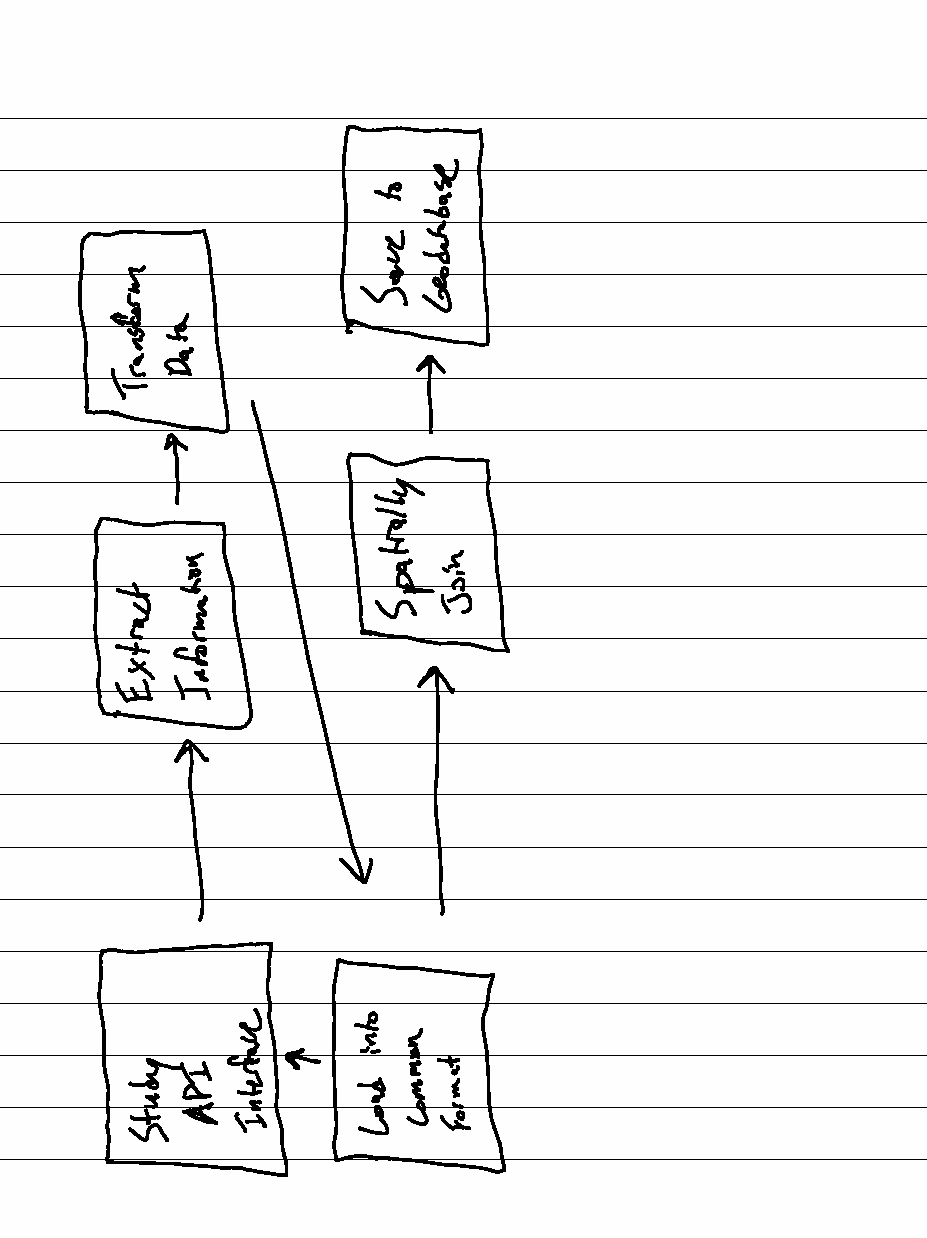
\includegraphics[width=.5\linewidth,angle=270]{steps}
			\end{minipage}
			\captionof{figure}{Project Steps}
		\end{center}
	\end{minipage}
}\\
{
	\scriptsize
	\begin{tabular}{|l|p{.2\linewidth}|p{.2\linewidth}|p{.2\linewidth}|p{.1\linewidth}|p{.1\linewidth}|p{.1\linewidth}|}
	\hline	& \textbf{Requirement} & \textbf{Defined As} & \textbf{(Spatial) Data} & \textbf{Attribute Data} & \textbf{Dataset} & \textbf{Preparation} \\ \hline
		1 & Model Traffic Emissions Dispersion         &                                                                & MnDoT’s Current AADT Segments           &                                                   & \href{https://gisdata.mn.gov/dataset/trans-aadt-traffic-segments}{MnDOT}                                                                                                                 &             \\ \hline
		2 & Model Industrial Emissions Dispersion      &                                                                & MPCA’s Permitted Facility Air Emissions &                                                   & \href{https://www.pca.state.mn.us/air/permitted-facility-air-emissions-data}{MPCA}                                                                                                      &             \\ \hline
		3 & Validate Models                            & Check model output with Observed data                          & PurpleAir                               & Pm2.5, VOCs ($\frac{\mu g}{m^3}$) & \href{https://api.purpleair.com/}{PurpleAir}                                                                                                                                                 &             \\ \hline
		4 & Synthesize Data                            & Ensure that all environmental risk variables are interoperable & Tree Canopy, Soil Data                  &                                                   & \url{http://doi.org/10.13020/D6C016}                                                                                                                                            &             \\ \hline
		5 & Experiment with Environmental Risk Indices & Experiment with different weights for variables                &                                         &                                                   &                                                                                                                                                                                                         &             \\ \hline
		6 & Correlation Analysis                       & Explore how variables/indices correlate                        & HOLC, Mapping Prejudice, Census         &                                                   & \href{https://gisdata.mn.gov/dataset/us-mn-state-metc-plan-historic-holc-appraisal}{HOLC} \newline  \href{https://mappingprejudice.umn.edu/racial-covenants/maps-data}{Mapping Prejudice} \newline \href{https://data2.nhgis.org/main}{Census} &             \\ \hline
		7 & Spatio-Temporal Modeling                   &                                                                &                                         &                                                   &                                                                                                                                                                                                         &       \\ \hline     
	\end{tabular}
\captionof{table}{Project Steps}}

\section*{Input Data}
{
	\scriptsize
	\begin{tabular}{|l|p{.2\linewidth}|p{.2\linewidth}|p{.4\linewidth}|}
	& \textbf{Title}                              & \textbf{Purpose in Analysis}     & \textbf{Link to Source}                                                               \\
	1 & MnDoT’s Current AADT Segments \cite{mndot_reg}     & Modeling and Risk Index & \url{https://gisdata.mn.gov/dataset/trans-aadt-traffic-segments}                   \\
	2 & MPCA’s Permitted Facility Emission \cite{mpca_emitter} & Modeling and Risk Index & \url{https://www.pca.state.mn.us/air/permitted-facility-air-emissions-data}        \\
	3 & PurpleAir Observed Air Quality    & Validating Model        & \url{https://api.purpleair.com/}                                                   \\
	4 & Tree Canopy \cite{tree2015}                        & Risk Index              & \url{http://doi.org/10.13020/D6C016}                                               \\
	5 & Soil Quality                       & Risk Index              &                                                                              \\
	6 & HOLC Grades                        & Correlation             & \url{https://gisdata.mn.gov/dataset/us-mn-state-metc-plan-historic-holc-appraisal} \\
	7 & Restrictive Deeds                  & Correlation             & \url{https://mappingprejudice.umn.edu/racial-covenants/maps-data}                \\
	8 & Demographics \cite{ipums}                       & Correlation             & \url{https://data2.nhgis.org/main}                                               
\end{tabular}
\captionof{table}{Data Sources}}

\section*{Methods}

To be determined... But for modeling air quality I'm considering using resources from both \href{https://www.pca.state.mn.us/business-with-us/air-quality-modeling}{MPCA}  and \href{https://plumepgh.org/model_data.html}{Plume Pittsburg}. I think the model validation will involve some RMSE, residual, and Pearson Correlation calculations. For the correlation analysis, I was thinking of doing something similar to an earlier project of mine using SLX, SLY, Durbin, and different GWR spatial regressions, but I'm open to suggestions! MPCA also has an \href{https://www.pca.state.mn.us/business-with-us/air-emissions-risk-analysis-aera}{air emissions risk assessment} that I will explore further when considering the risk index.

\section*{Results}

\begin{adjustwidth}{-.55in}{-.55in}	
	\fbox{ % Fig Naphthalene Interpolations
			\begin{minipage}{.5\linewidth}
				\begin{center}
					\begin{minipage}{\linewidth}
						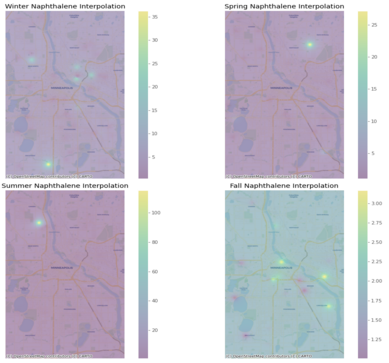
\includegraphics[width=\linewidth]{Naphthalene Interpolations.png}
					\end{minipage}
					\captionof{figure}{The seasonal interpolations of Naphthalene readings ($\mu g/m^3$).}
				\end{center}
			\end{minipage}
		
	}
	\\
	\fbox{\begin{minipage}{\linewidth} % Figure - Benzene Raw
			\hspace{1in}
			\begin{minipage}{.5\linewidth}
				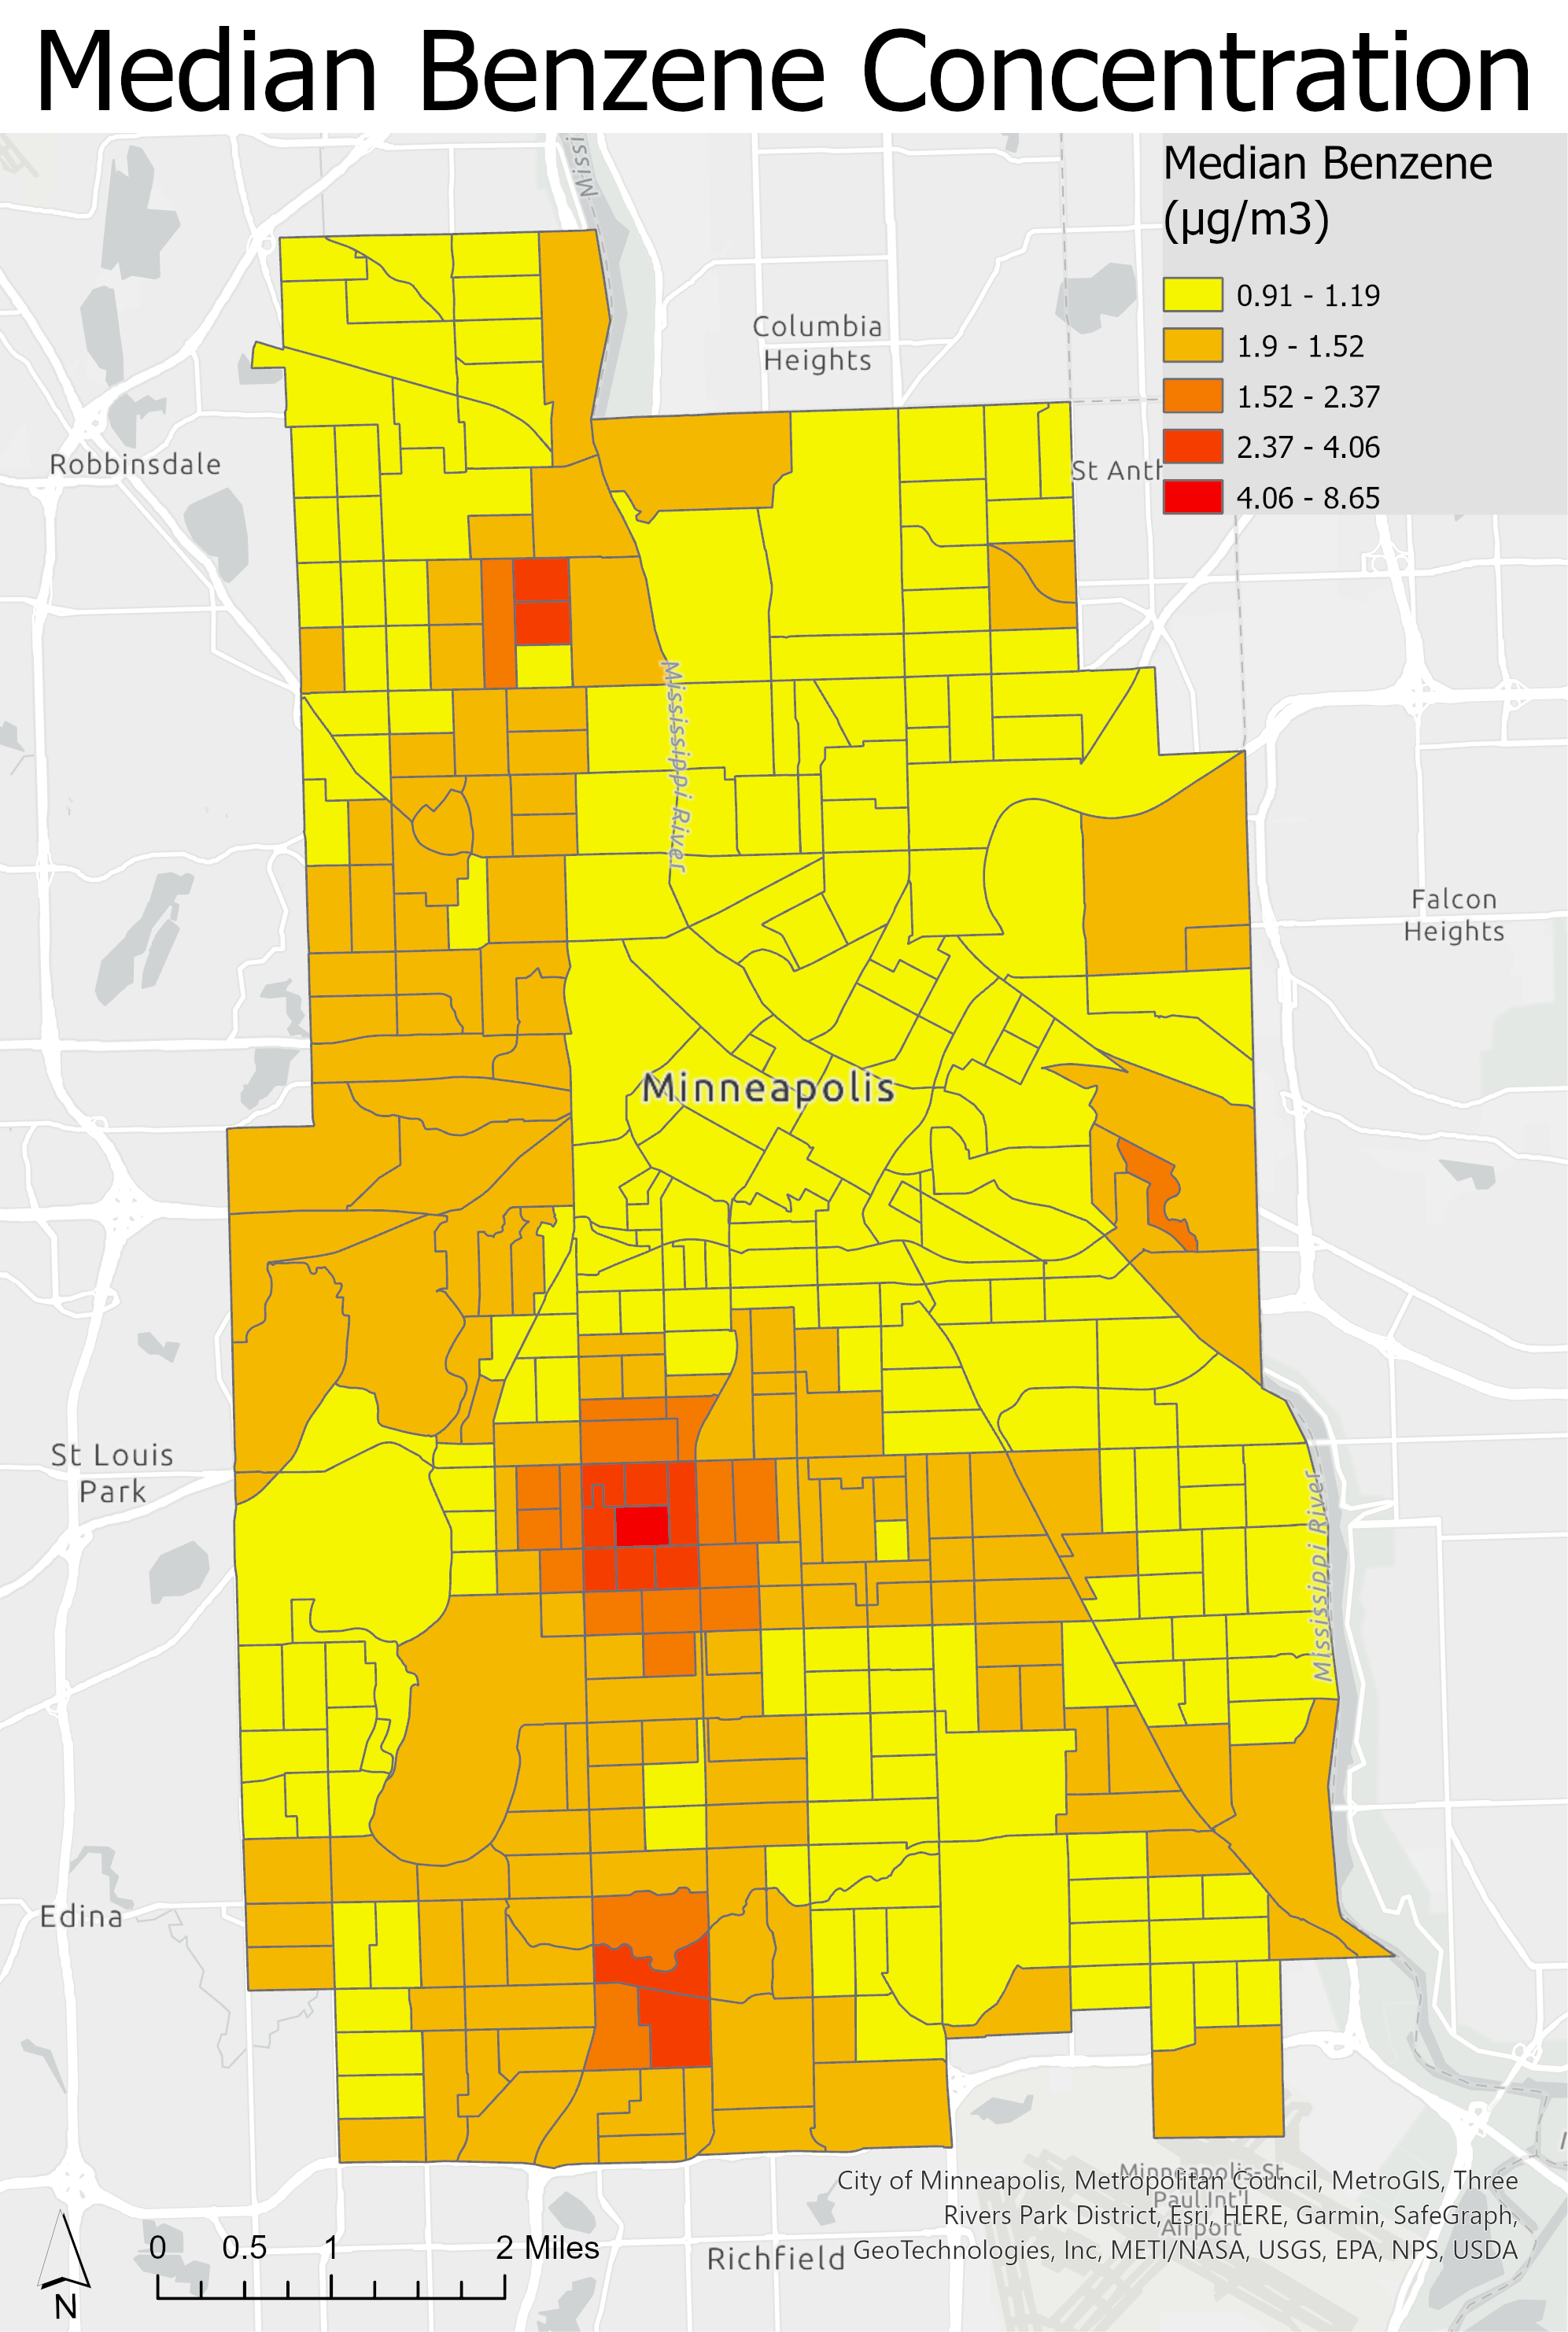
\includegraphics[width=.4\linewidth]{median_benzene_concentration}
			\end{minipage} % Figure - Naphthalene Raw
			\begin{minipage}{.5\linewidth}
				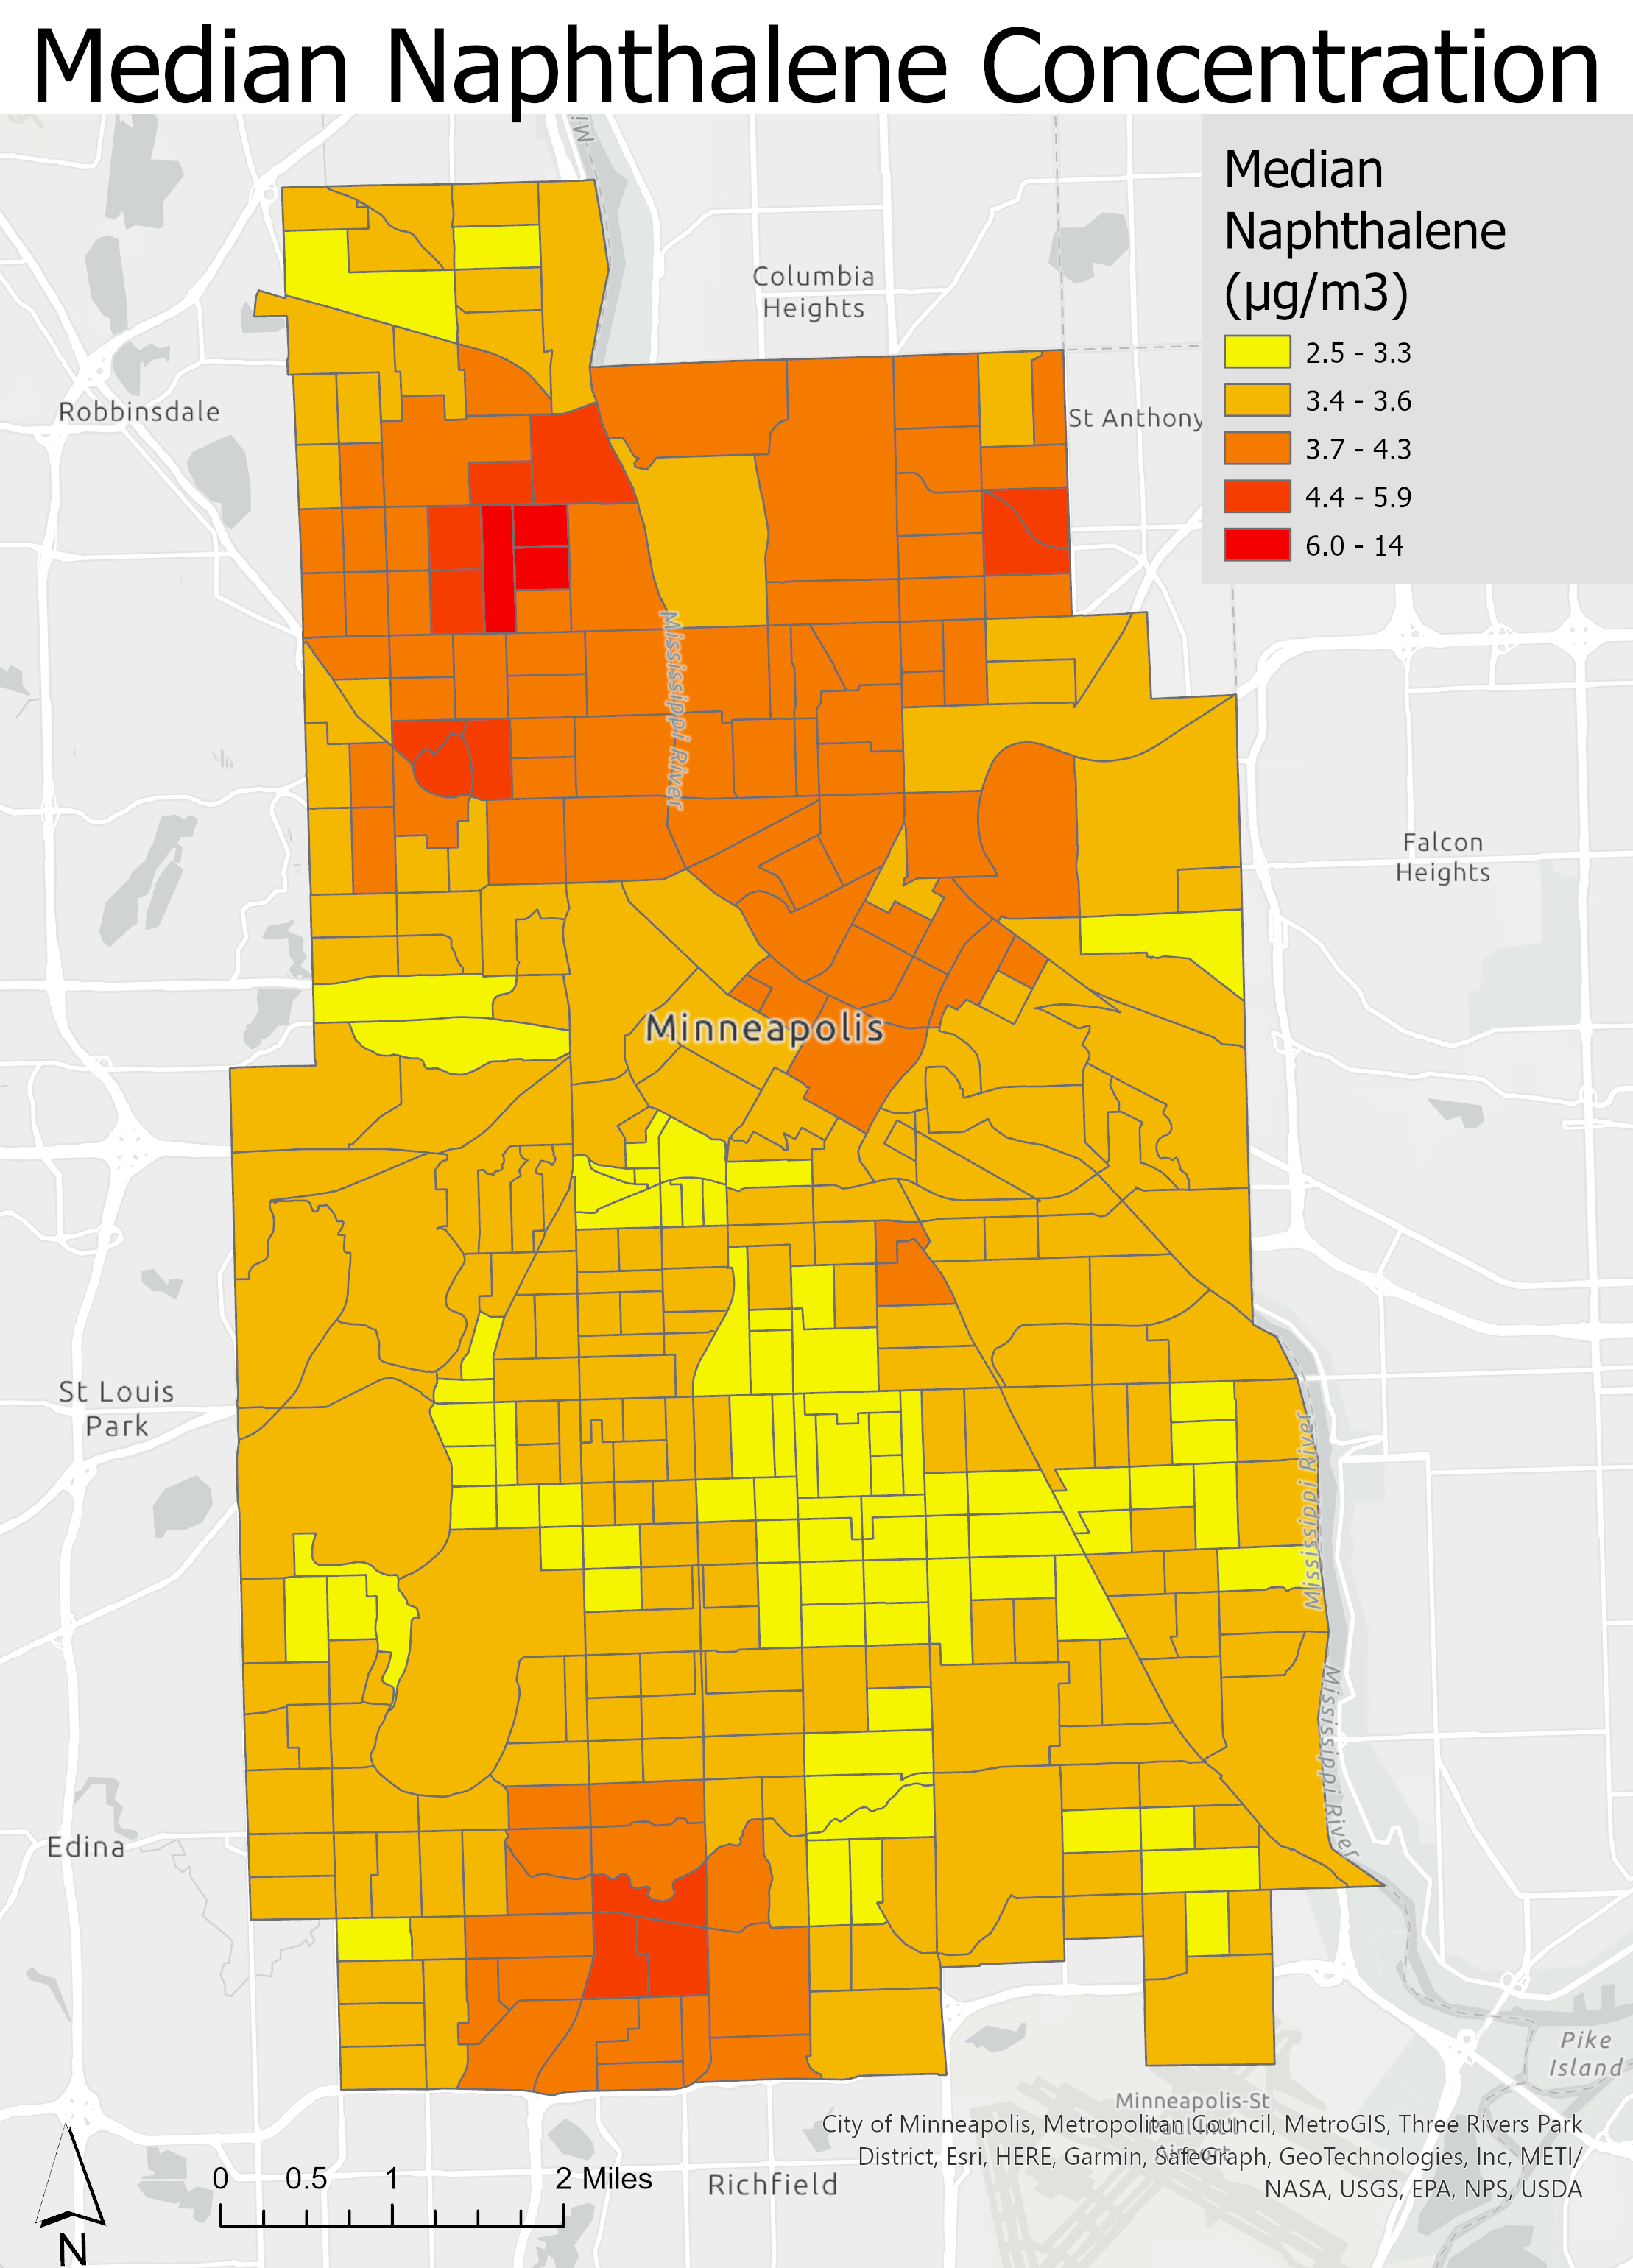
\includegraphics[width=.42\linewidth]{median_naphthalene_concentration}
			\end{minipage}
			\captionof{figure}{Visualizations of zonal statistics of volatile organice compounds by block group.}
	\end{minipage}}
	
\end{adjustwidth}

\begin{adjustwidth}{-.55in}{-.55in}
	\begin{center}
		\fbox{
			\begin{minipage}{\linewidth}
				\captionof{figure}{Geographically weighted regressions (Air Quality). Fixed 2 kilometer bandwidth.}
				\begin{center}	
					\fbox{ % Figure - Benzene GWR - All
						\begin{minipage}{.5\linewidth}
							\begin{center}
								\begin{minipage}{\linewidth}
									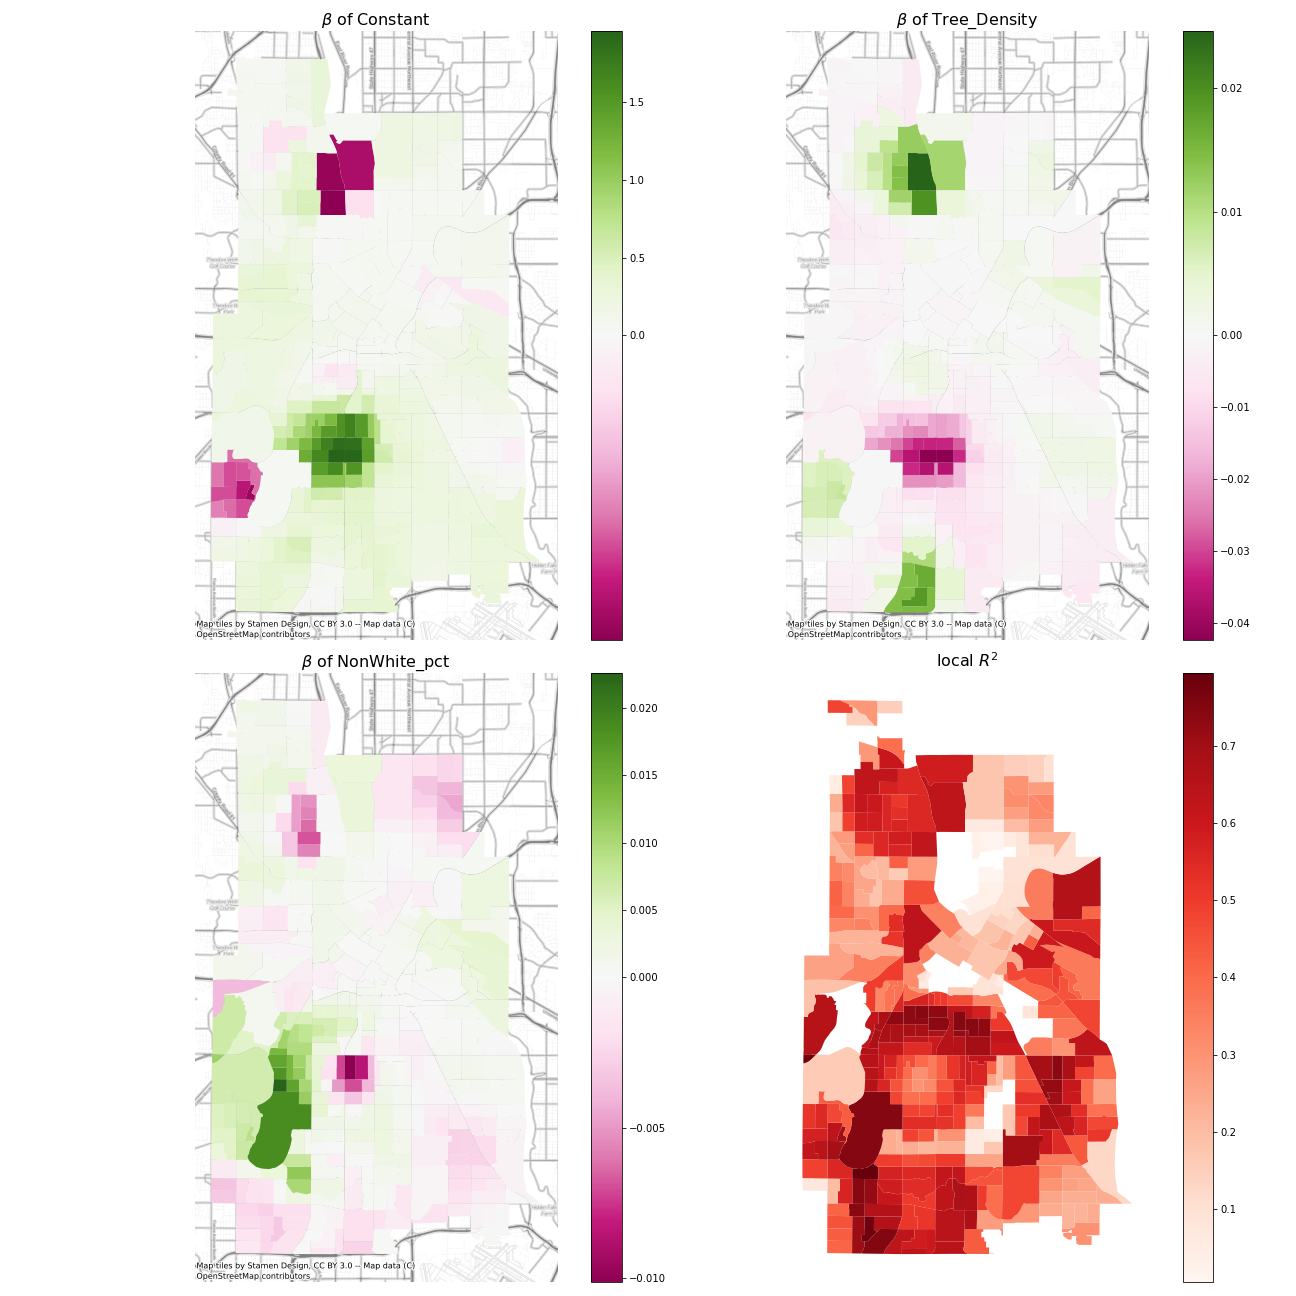
\includegraphics[width=\linewidth]{Benzene GWR - All Variables}
								\end{minipage}
								\captionof*{figure}{Regressand: $A_B$, Regressor: $T$ and $R_{NW}$.}
							\end{center}
						\end{minipage}
					}
				\end{center}
				
				\begin{center}	
					\fbox{ % Figure - Naphthalene GWR - All
						\begin{minipage}{.5\linewidth}
							\begin{center}
								\begin{minipage}{\linewidth}
									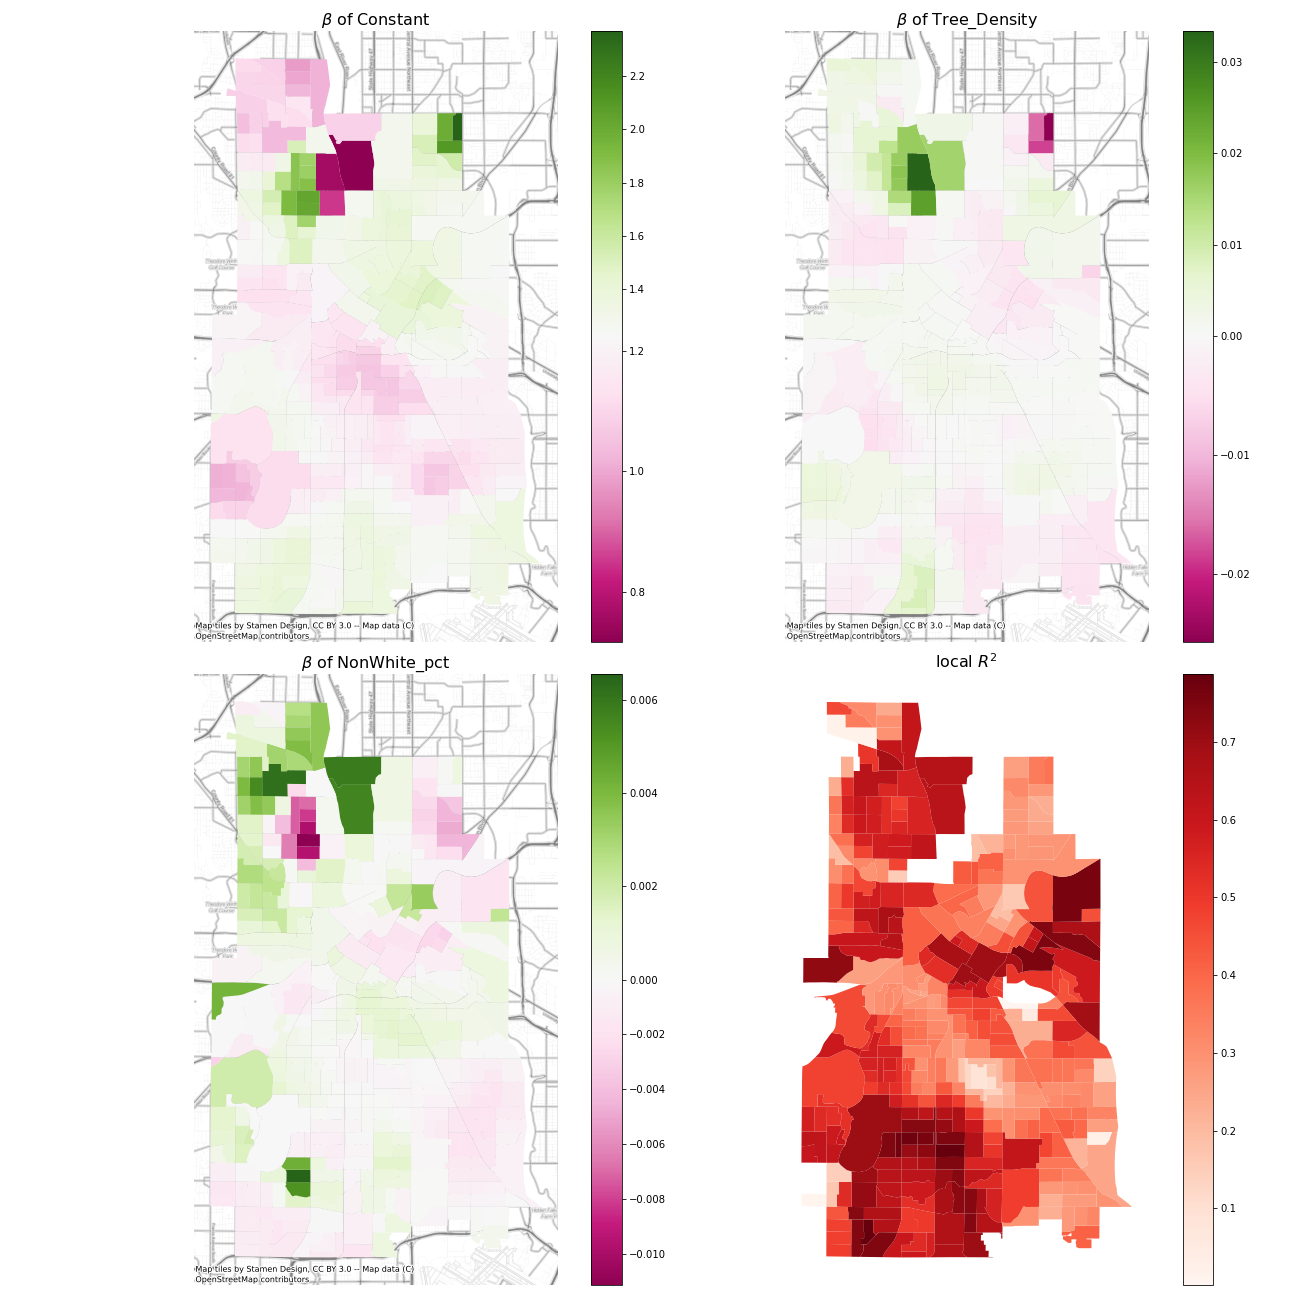
\includegraphics[width=\linewidth]{Naphthalene GWR - All Variables}
								\end{minipage}
								\captionof*{figure}{Regressand: $A_N$, Regressor: $T$ and $R_{NW}$.}
							\end{center}
						\end{minipage}
					}
				\end{center}
		\end{minipage}}	
		
	\end{center}
\end{adjustwidth}

\begin{tabular}{lrrrrr}
	\hline
	{} &     $R^2$ &  Pearson Coeff &     p-value &  Residual Morans I &     p-value \\
	\hline
	NonSpatial &  0.0888 &         0.2980 &  3.7698e-09 &             0.4336 &  1.1466e-18 \\
	SLX        &  0.1041 &         0.3226 &  1.4926e-10 &             0.4393 &  3.5773e-19 \\
	SLY        &  0.2682 &         0.5179 &  3.4336e-27 &            -0.0877 &  8.9419e-02 \\
	Durbin     &  0.2673 &         0.5170 &  4.3190e-27 &            -0.0774 &  1.3412e-01 \\
	GWR        &  0.4777 &         0.6959 &  9.7322e-56 &            -0.4243 &  7.2401e-18 \\
	\hline
\end{tabular}
\captionof{table}{Accuracy checks of regressions. Regressand: $T$, Regressor: $R_{NW}$.}
\vspace{.2in}
\begin{adjustwidth}{-.55in}{}
	\begin{tabular}{lrrrrllll}
		\hline
		{} &  CONSTANT &       p-value &  $R_{NW}$ &      p-value & $R_{NW}$\_lag &  p-value & $T$\_lag & p-value \\
		\hline
		NonSpatial &  33.44931 &  1.98079e-135 &      -0.12088 &  3.76979e-09 &                - &        - &              - &       - \\
		SLX        &  34.99942 &  8.84001e-115 &      -0.05236 &  1.21008e-01 &         -0.11258 &  0.01219 &              - &       - \\
		SLY        &  12.48954 &   5.28596e-07 &      -0.05557 &  3.39681e-03 &                - &        - &        0.63771 &     0.0 \\
		Durbin     &  13.00777 &   4.13289e-06 &      -0.04503 &  1.39290e-01 &         -0.01866 &  0.65725 &        0.62976 &     0.0 \\
		\hline
	\end{tabular}
	\captionof{table}{Coefficients of regression models. Regressand: $T$, Regressor: $R_{NW}$.}
	
\end{adjustwidth}



\section*{Results Verification}

The air quality modeling will be verified with the observations from PurpleAir Sensors. Literature will be consulted on how best to construct and refine an index. 

\section*{Discussion and Conclusion}

	Environmental justice (EJ) continues to expand and incorporate different conceptions of space, environment, and justice. Contemporary EJ writers often cite a need for more community outreach, education, and inclusive decision-making as well as innovative collaboration between planners, policy-makers, academics, and citizens to achieve profound environmental justice \cite{walker2010, corburn2003, pearsall2010}. \textcite{pearsall2010} emphasize a need for well defined indicators that are spatially focused, not aggregate measures, to gauge a policy's success at implementing environmental justice. This new workflow and index are a couple more tools we can use to collectively reckon with our history, assess our current situation, and work toward reparations. 

\begingroup           % Ctrl T to uncomment
\setstretch{1}
\setlength\bibitemsep{12pt}  % length between two different entries
\printbibliography
\endgroup

\section*{Self Score}
\setstretch{.2}
\begin{tabular}{|p{.2\linewidth}|p{.2\linewidth}|p{.2\linewidth}|p{.1\linewidth}|}
	\hline
	\textbf{Category}            & \textbf{Description}                                                                                                                                                                                                                                                                                                                                              & \textbf{Points Possible} & \textbf{Score} \\ \hline
\vspace{.2in}\textbf{Structural Elements} & {\tiny All elements of a lab report are included (2 points each): Title, Notice: Dr. Bryan Runck, Author, Project Repository, Date, Abstract, Problem Statement, Input Data w/ tables, Methods w/ Data, Flow Diagrams, Results, Results Verification, Discussion and Conclusion, References in common format, Self-score}                                        & \vspace{.2in}28              &   \vspace{.2in}24    \\ \hline
	\vspace{.2in}\textbf{Clarity of Content}  & {\tiny Each element above is executed at a professional level so that someone can understand the goal, data, methods, results, and their validity and implications in a 5 minute reading at a cursory-level, and in a 30 minute meeting at a deep level (12 points). There is a clear connection from data to results to discussion and conclusion (12 points).} & \vspace{.2in}24              &  \vspace{.2in}22     \\ \hline
	\vspace{.2in}\textbf{Reproducibility}     & {\tiny Results are completely reproducible by someone with basic GIS training. There is no ambiguity in data flow or rationale for data operations. Every step is documented and justified.}                                                                                                                                                                     & \vspace{.2in}28              &     \vspace{.2in}24  \\ \hline
	\vspace{.2in}\textbf{Verification}        & {\tiny Results are correct in that they have been verified in comparison to some standard. The standard is clearly stated (10 points), the method of comparison is clearly stated (5 points), and the result of verification is clearly stated (5 points).}                                                                                                      & \vspace{.2in}20              &   \vspace{.2in}20    \\ \hline
	&                                                                                                                                                                                                                                                                                                                                                          & \vspace{.02in}100             &   \vspace{.02in}90     \\ \hline
\end{tabular}
\end{document}